\subsubsection{Prometheus}\label{prom}
Prometheus was integrated into both the API and the application through a custom middleware that intercepts HTTP requests to gather metrics. The metrics collected includes:

\begin{itemize}
\item \texttt{http\_requests\_total}: A counter that counts the total number of HTTP requests. It includes labels for request path, HTTP method, and status code. This metric helped us monitor request load per endpoint, track response statuses (in general or just on an endpoint basis).
\item \texttt{http\_request\_duration\_seconds}: A histogram measuring the time taken to process HTTP requests, in seconds. It is labeled by request path and method, enabling performance benchmarks for endpoints.
\item \texttt{http\_response\_messages\_total}: A counter that logs the total number of HTTP responses, categorized by status code and message type. Before logging was fully implemented, this metric was particularly helpful in identifying which endpoints triggered specific status messages and understanding the reasons behind them. A bit deprecated as soon as logging was implemented.
\end{itemize}
Seen in retrospect, it would have been a good idea also to collect metrics on database queries, but this will be described more thoroughly in section \ref{maintainence}

\subsubsection{Grafana}
While Prometheus was important for collecting data, Grafana was utilized to visualize the data. Grafana connects to Prometheus as a data source, enabling the creation of dashboards. As mentioned in section \ref{prom}, we monitored both our API and app, which resulted in us setting up two dashboards: one for the app and one for the API (see figure \ref{fig:monitoring}).
\\\\
For instance, the API dashboard converted the metrics collected by Prometheus into a clear visual representation of the API's health and performance. Panels were set up to showcase:
\begin{itemize}
    \item Indicators from \texttt{http\_requests\_total}, such as the rate of requests per second, overall request load distributed by endpoint, and the ratio of successful and client-error status codes.
    \item Performance monitored by \texttt{http\_request\_duration\_seconds}, including average response times and 99th percentile latency, allowing for quick identification of performance degradation.
\end{itemize}

\begin{figure}[h]
\centering
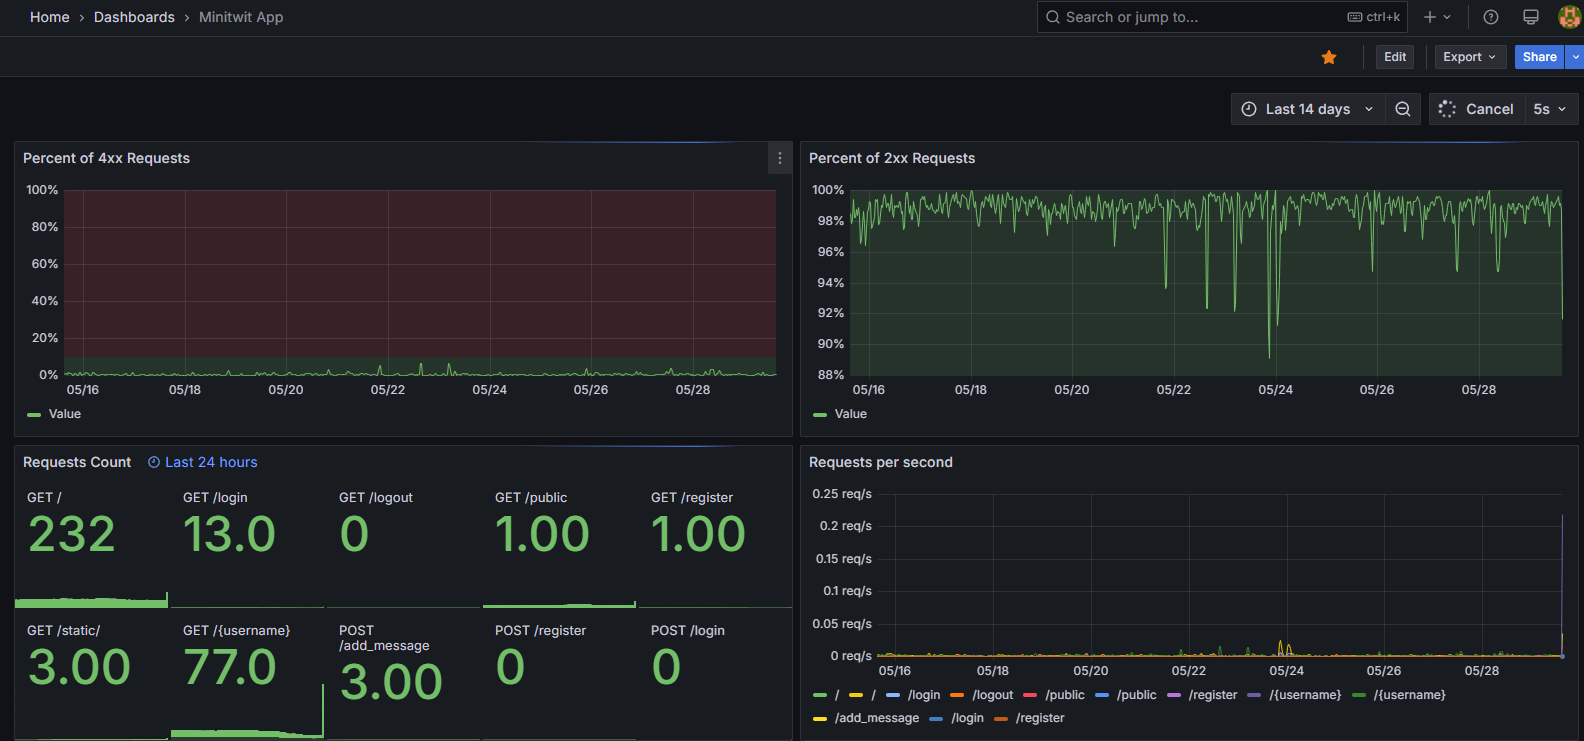
\includegraphics[width=\textwidth]{images/metrics.png}
\caption{A snippet of our App dashboard in Grafana}
\label{fig:monitoring}
\end{figure}